%!TEX root =  ../final-report.tex

% Chapters are setup to start on a new page.
% The short version of that title appears in square brackets. This is used for the table of contents listing. 
% The long version of the title has a command "\setstretch{0.5}" in order to reduce the line spacing in the
% title and then the title text.

\section{H-field Antenna}

\subsection{Purpose}

Normally microwave imaging systems consist of a simple E-field antenna such and a Monopole or a Dipole antenna which has one polarization and it is limited in its functionality, however it is simple to model in the imaging inversion algorithm as these types of antennas have very simple and well defined current distributions along them. Due to a grain storage bin being round, metallic, and closed off at both ends, it can be thought of as a cylindrical resonant chamber which introduces a level of difficulty in designing antennas that can operate in such an environment. However since the walls of the bin are metallic, the field components at the metallic walls are easily differentiable, the H-fields are tangential to the metallic walls of the chamber, and the E-fields are perpendicular to the walls, thus we would like to have an antenna that is capable of probing the tangential H-fields only.

The H- field antenna design had to be confined to the following design criteria in order for it to be effective inside of the grain bin:

\begin{itemize*}

\item Ability to pick up H-field only, and reject most of the E-field
\item Minimal size (less that 15cm in length or witdth)ˆ
\item Frequency of operation between 70Mhz-90Mhzˆ
\item Matched to 50 ohm coaxial transmission lineˆ
\item Physically able to withstand grain being filled into the binˆ
\item Reduced complexity(for ease of modeling in the inversion algorithm)ˆ
\item Ease of manufacturing and reproduction

\end{itemize*}

\subsection{Research}

The typical design procedure for an H-field antenna is a loop of perimeter one $\lambda$ as at that length the loop becomes purely resistive with the maximum amount of radiation resistance, however this approach does not work for the grain bin as the perimeter of the loop would have to be almost 4 meters.

The other typical approach to designing h-field antennas is to decrease the perimeter of the loop and increase the number of turns which allows for the required size reduction that we are looking for as well as enable it to be matched to a 50ohm coaxial line since the radiation resistance is proportional to the number of turns squared $R_r = (\frac{177NS}{\lambda})^2$, however it is also not feasible for the grain bin since it would not guarantee that the antenna does not pick up the E-field as well, and it would be too complex to model in the imaging software.

\subsection{Design}

In order to satisfy the main requirement of the antenna (1) a shielded and slotted loop antenna was chosen, which is a common type of antenna used in radio.

\begin{figure}[h]
	\begin{center}
		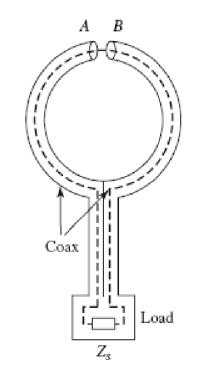
\includegraphics[width=1.5in]{./images/Figure1.jpg}
		\caption{}
		\label{fig:hfield_fig1}
	\end{center}
\end{figure}

The ground layer around the conductor which acts as the shielding modifies the electric field distribution inside of the antennas cross sectional area due to the boundary conditions on a PEC, thus reducing its effect on the antenna, this effect is confirmed in the simulation results in section \ref{sec:sim_results}. Since the magnetic field passing through the loop induces a current on both the conductor and the shielding, a slot is cut out in the shield to create a capacitance which introduces a phase shift between the two currents and therefore there is a difference in potential across the load.

The second requirement (2) was met by reducing the perimeter of the antenna to $\lambda /20$, however the small size presented another challenge which is matching the loop antenna to the 50ohm coaxial line, different ways of matching were considered such as capacitive coupling and transformer coupling between the coaxial line and the antenna, These were simulated in HFSS but found the it would be too complex to build accurately, and it would not be feasible to mount in the grain bin. Mohammad (Project co-supervisor) suggested the use of a 50ohm termination at the end of the loop to match the antenna to a 50ohm line and to cut the loop in half so that the size of it could be further reduced as well as to take advantage of having a metallic wall as the other half of the loop. A prototype of this antenna was built using a semi rigid coaxial cable with a slot cut in the ground conductor and a 50 ohm termination was used to match the antenna to a coaxial line.

\begin{figure}[h]
	\begin{center}
		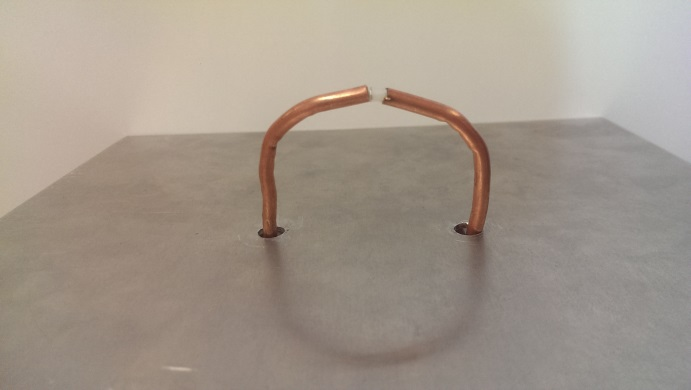
\includegraphics[width=4in]{./images/Figure2.jpg}
		\caption{prototype antenna}
		\label{fig:hfield_fig2}
	\end{center}
\end{figure}

A difference of 10db was observed between the E and H polarization. However building multiples of such antennas accurately would not be feasible since the slot size would vary and produce inaccurate results as well as the curvature in the antenna is tough to reproduce accurately.

In order to make the antenna easy to manufacture and reproduce, it was decided that a PCB version would be best suitable.

\subsection{PCB Antenna Design}

To achieve a shielded coaxial line on PCB, a groundless co-planar waveguide was chosen, due to material availability, 0.8mm FR-4 material was chosen as the PCB material with a relative permittivity of 4.3. Due to the limited capabilities of the PCB prototyping machine available at the EIL lab, a minimum cut in the PCB could not exceed 0.2mm, therefore 0.2mm was chosen as the gap between the conductor and the ground planes of the co-planar waveguide. With the help of TX-line (transmission line calculation software) a conductor size of 2.57mm with a gap of 0.2mm and a 0.8mm FR-4 thickness yields the necessary 50ohm transmission line. The size of the antenna is 12.5cm in length and 5.5cm in width with 45 degree bends for reducing reflections, the bent sections are 1cm long.

\subsection{PCB Antenna Simulation}

The PCB version of the antenna is constructed in the high frequency structure simulator with FR-4 as the substrate material, copper material on top of the substrate is simulated as perfect conductor and an infinite ground plane as the antennas backing plate. The design is simulated and optimized to obtain its performance characteristics. From optimization a slot size of 1 mm is chosen in the shielding.

\begin{figure}[h]
	\begin{center}
		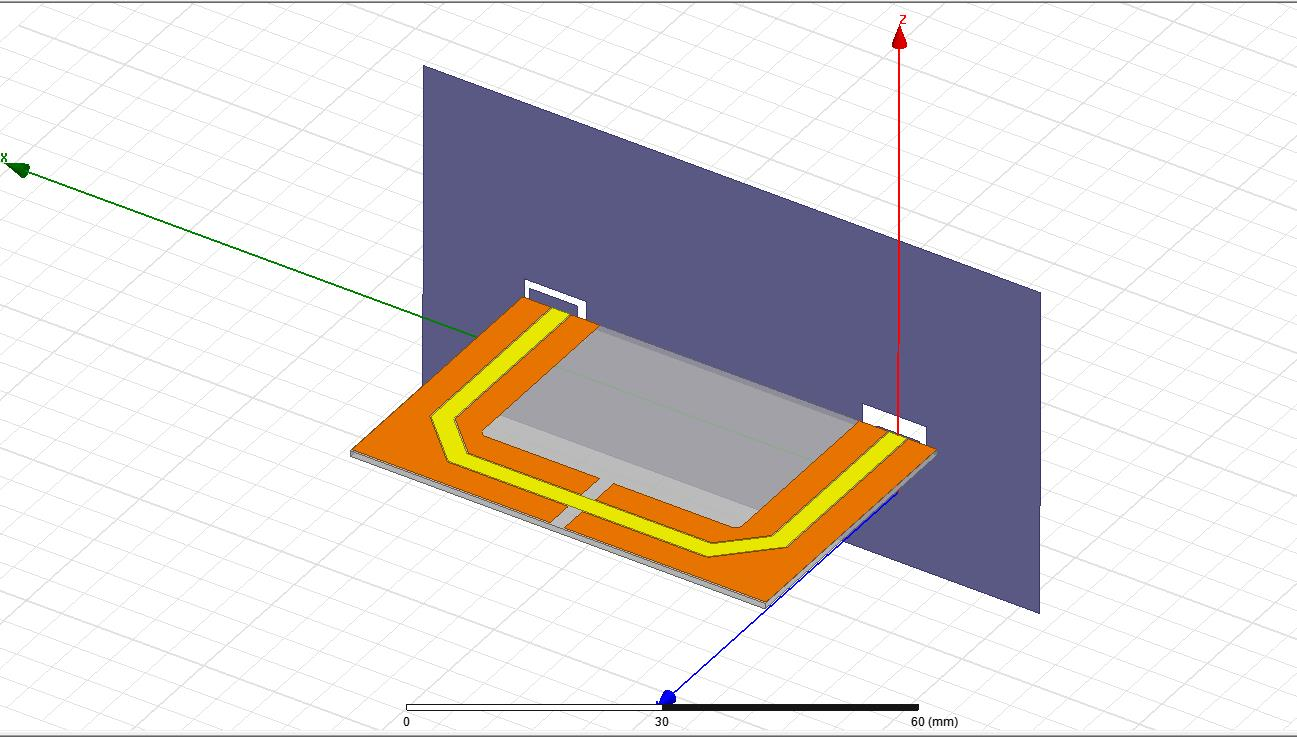
\includegraphics[width=4in]{./images/Figure3.jpg}
		\caption{HFSS model}
		\label{fig:hfield_fig3}
	\end{center}
\end{figure}

\subsection{Simulation Results}
\label{sec:sim_results}

The desired result is to have an S11 (insertion loss) of -10db at the frequency of operation, and as expected the insertion loss at 80 MHz is -14.5db as well as due to the 50 ohm termination the antenna has a really high bandwidth.

The simulation also confirms the effect of the co-planar ground plane on the Electric fields inside the cross sectional area of the antenna, Figure 6 and Figure 7 show the antenna with shielding and antenna without shielding E-field magnitude distribution in the cross sectional area.

\begin{figure}[h]
	\begin{center}
		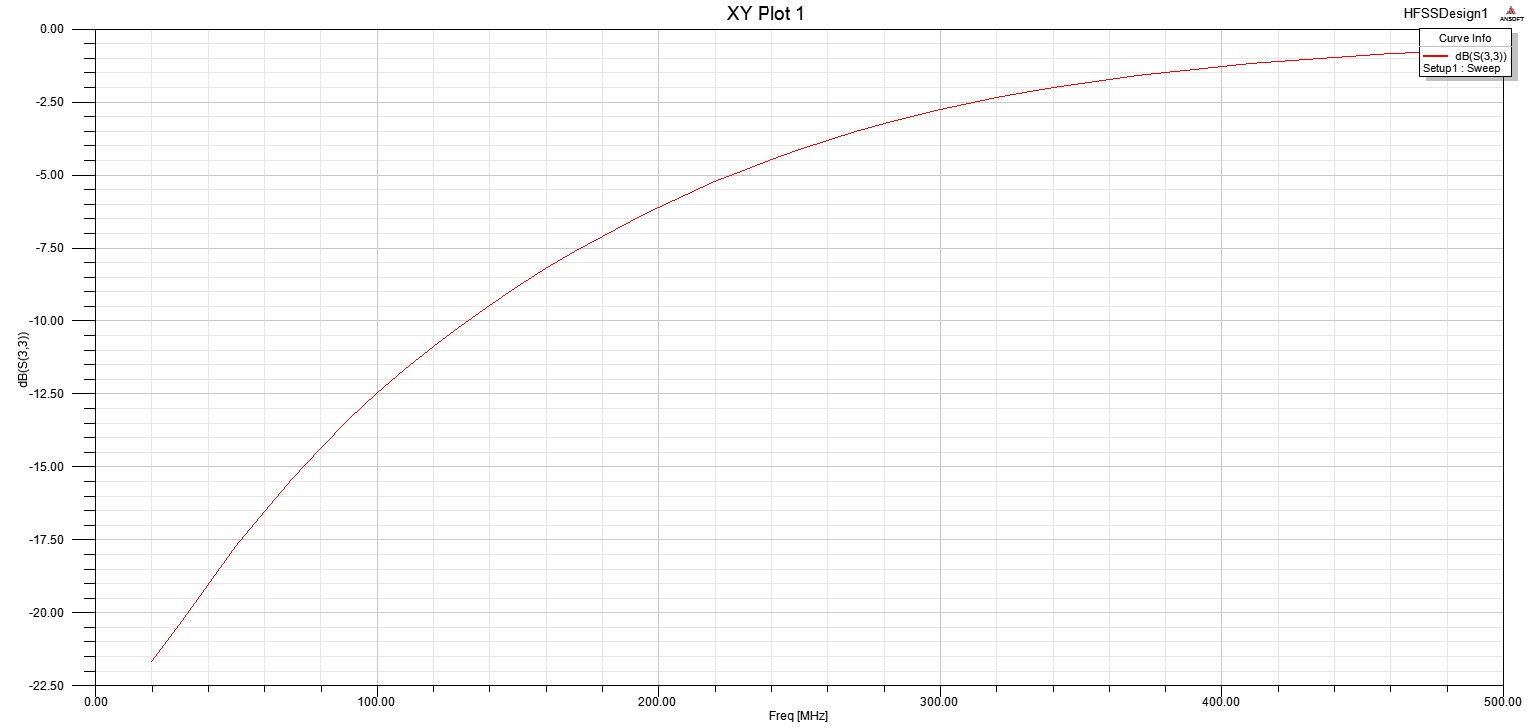
\includegraphics[width=5in]{./images/Figure4.jpg}
		\caption{S11}
		\label{fig:hfield_fig4}
	\end{center}
\end{figure}

\begin{figure}[h]
	\begin{center}
		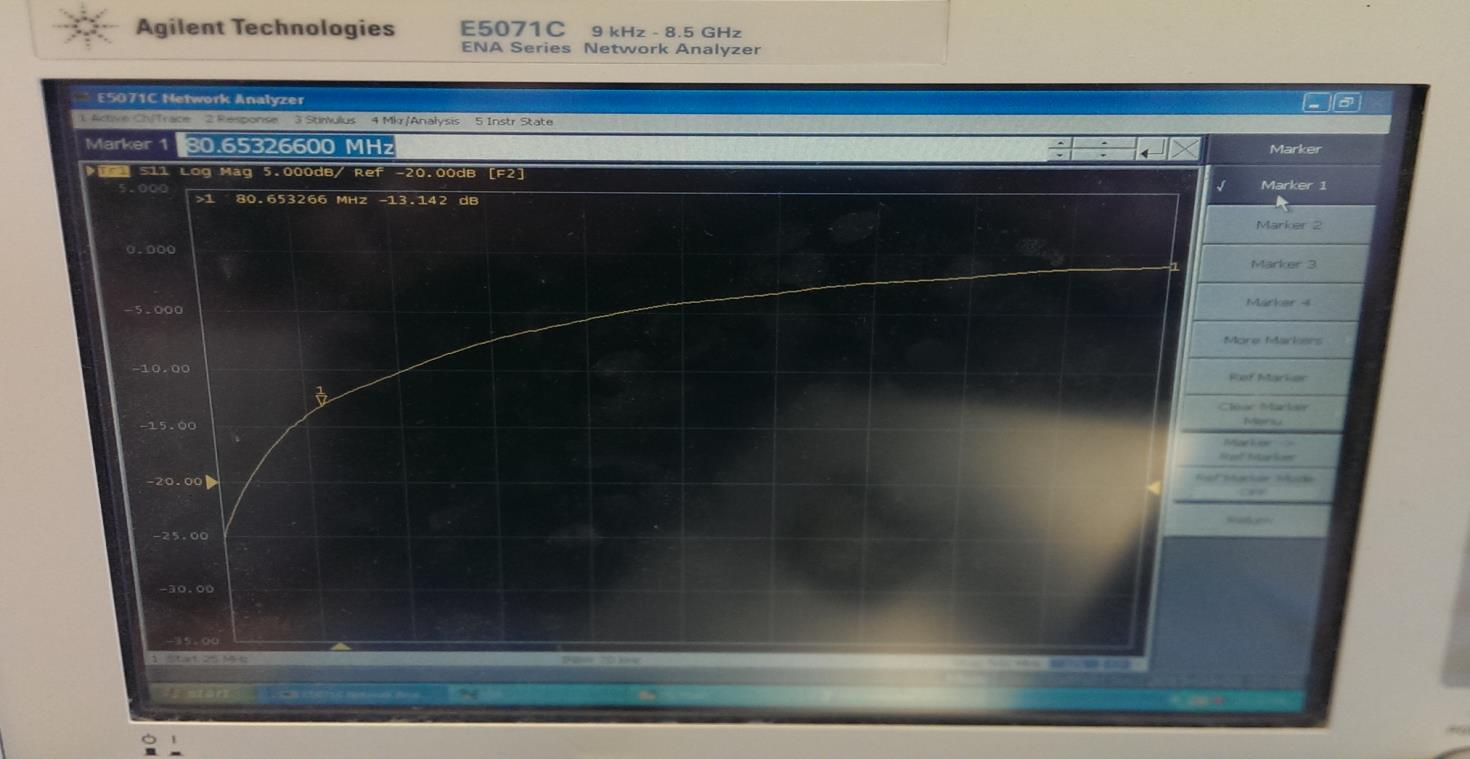
\includegraphics[width=5in]{./images/Figure5.jpg}
		\caption{Built antenna S11}
		\label{fig:hfield_fig5}
	\end{center}
\end{figure}

\begin{figure}[h]
	\begin{center}
		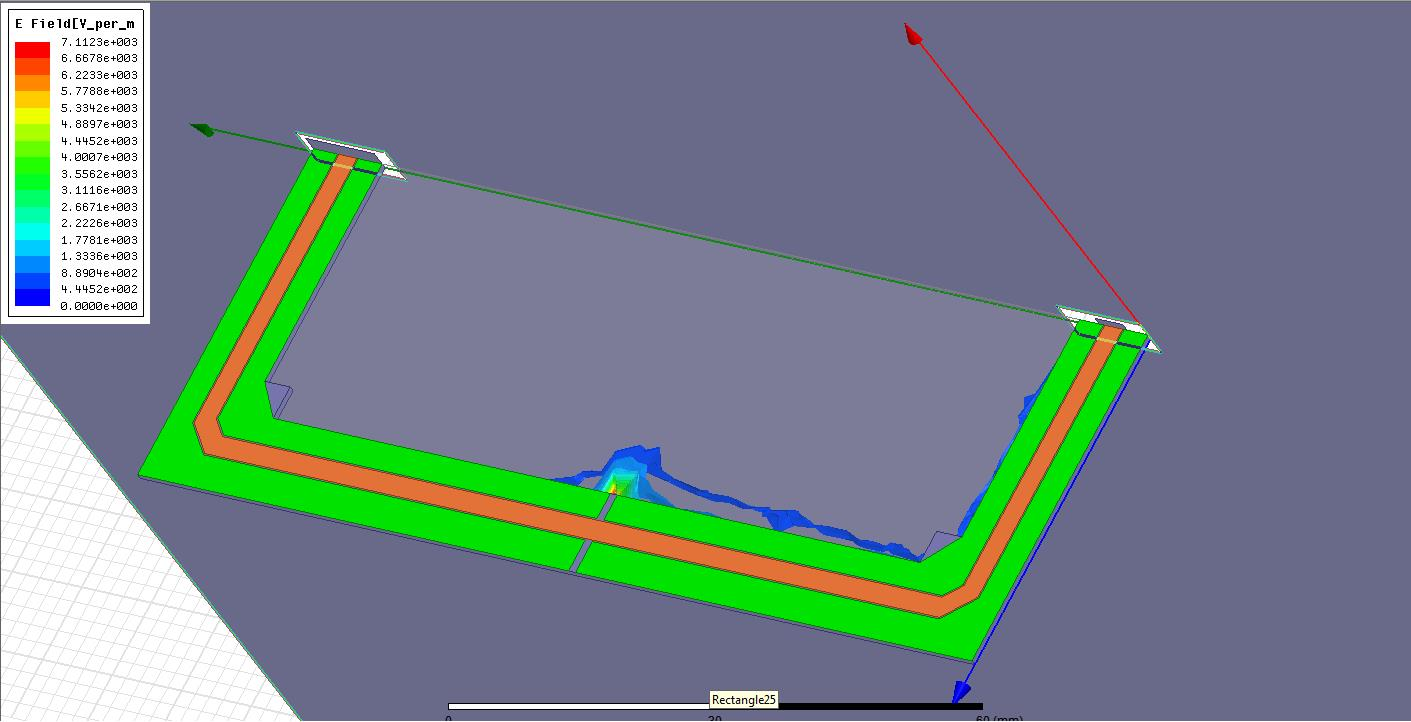
\includegraphics[width=4in]{./images/Figure6.jpg}
		\caption{Loop antenna with shielding}
		\label{fig:hfield_fig6}
	\end{center}
\end{figure}

\begin{figure}[h]
	\begin{center}
		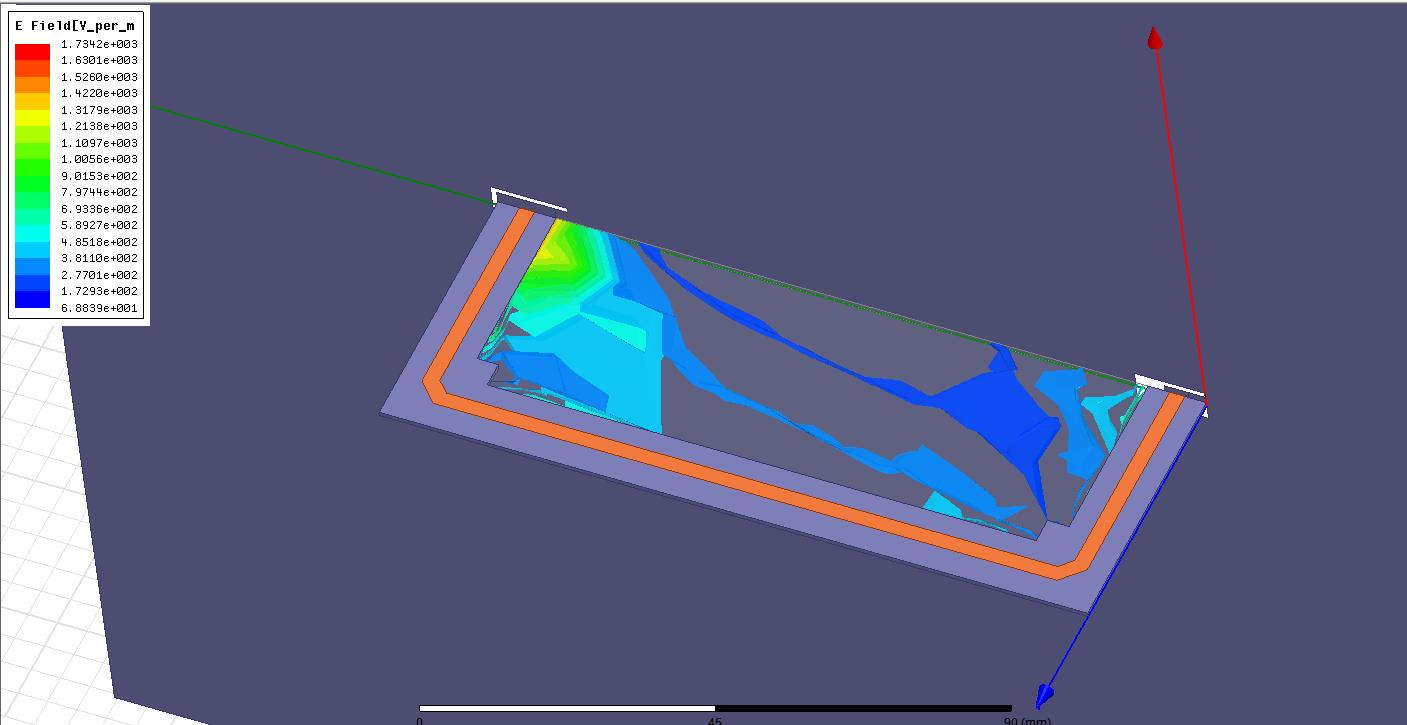
\includegraphics[width=4in]{./images/Figure7.jpg}
		\caption{Shielding removed}
		\label{fig:hfield_fig7}
	\end{center}
\end{figure}

\subsection{PCB Layout}

After simulating the antenna in HFSS, the design was transferred to Altium which was used to create the necessary Gerber files for fabrication. The antenna was fabricated in the EIL with the use of the rapid PCB prototyping machine.

\begin{figure}[h]
	\begin{center}
		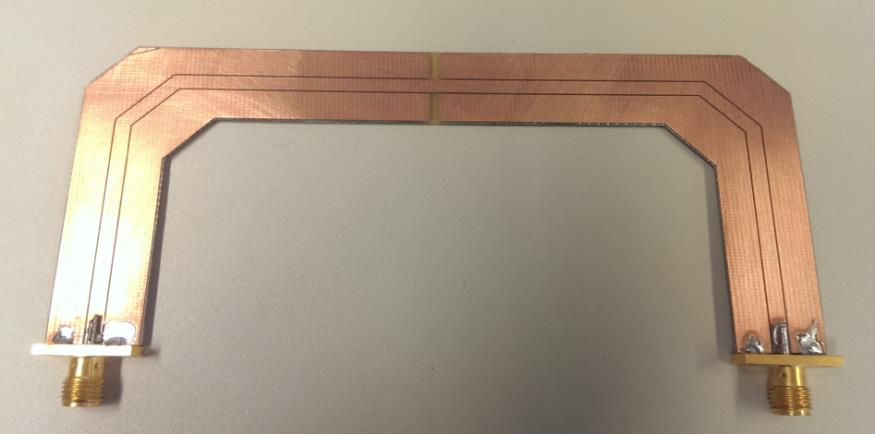
\includegraphics[width=4in]{./images/Figure8.jpg}
		\caption{fabricated antenna}
		\label{fig:hfield_fig8}
	\end{center}
\end{figure}

\subsection{H-field Antenna Testing}

The antenna’s ability to reject the Electric field was tested in a G-TEM cell. The G-TEM cell creates transverse EM waves guided between a pair of plates with H orthogonal to E, the incident wave was created with a signal generator producing an 80 MHz sine wave with 0dbm power and the AUT measurements were taken with a spectrum analyzer. Two orientations of the antenna were tested in the cell, longitudinally parallel with the magnetic field (E-orientation) and perpendicular to magnetic field (H-orientation).

\begin{figure}[h]
	\begin{center}
		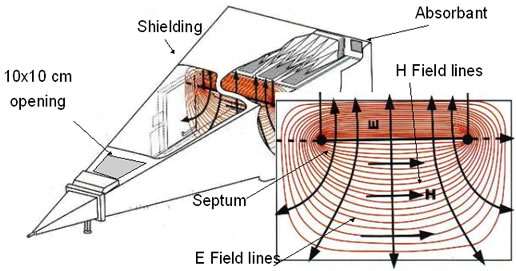
\includegraphics[width=4in]{./images/image9.jpeg}
		\caption{field lines in G-TEM for reference}
		\label{fig:hfield_fig9}
	\end{center}
\end{figure}

\subsection{G-TEM Test Results}

The noise floor of the antenna was measured at -83dbm with incident power of -13dbm.

When oriented in the E-orientation the antenna received -81dbm which is close to the noise level of the antenna, when oriented in the H-orientation the antenna received -65dbm therefore a difference of 16db exists between the two orientations which shows that the antenna is picking up only H-field.

\begin{figure}[h]
	\begin{center}
		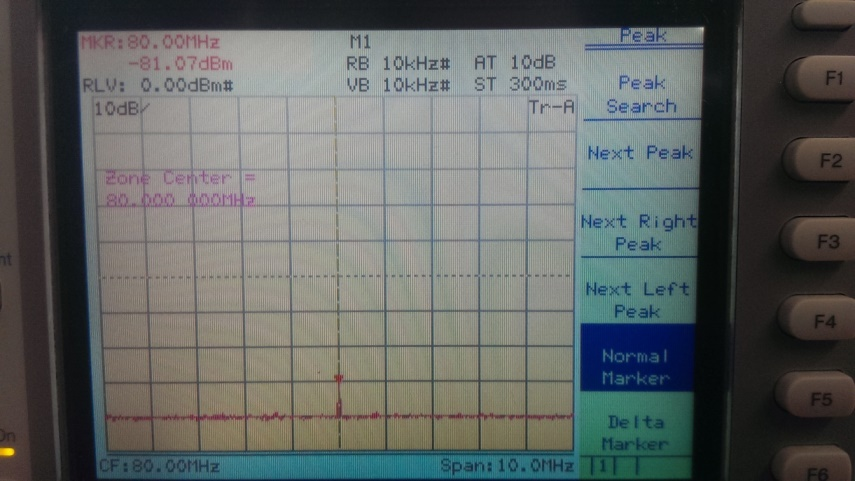
\includegraphics[width=4in]{./images/Figure9.jpg}
		\caption{E-orientation}
		\label{fig:hfield_fig10}
	\end{center}
\end{figure}

\begin{figure}[h]
	\begin{center}
		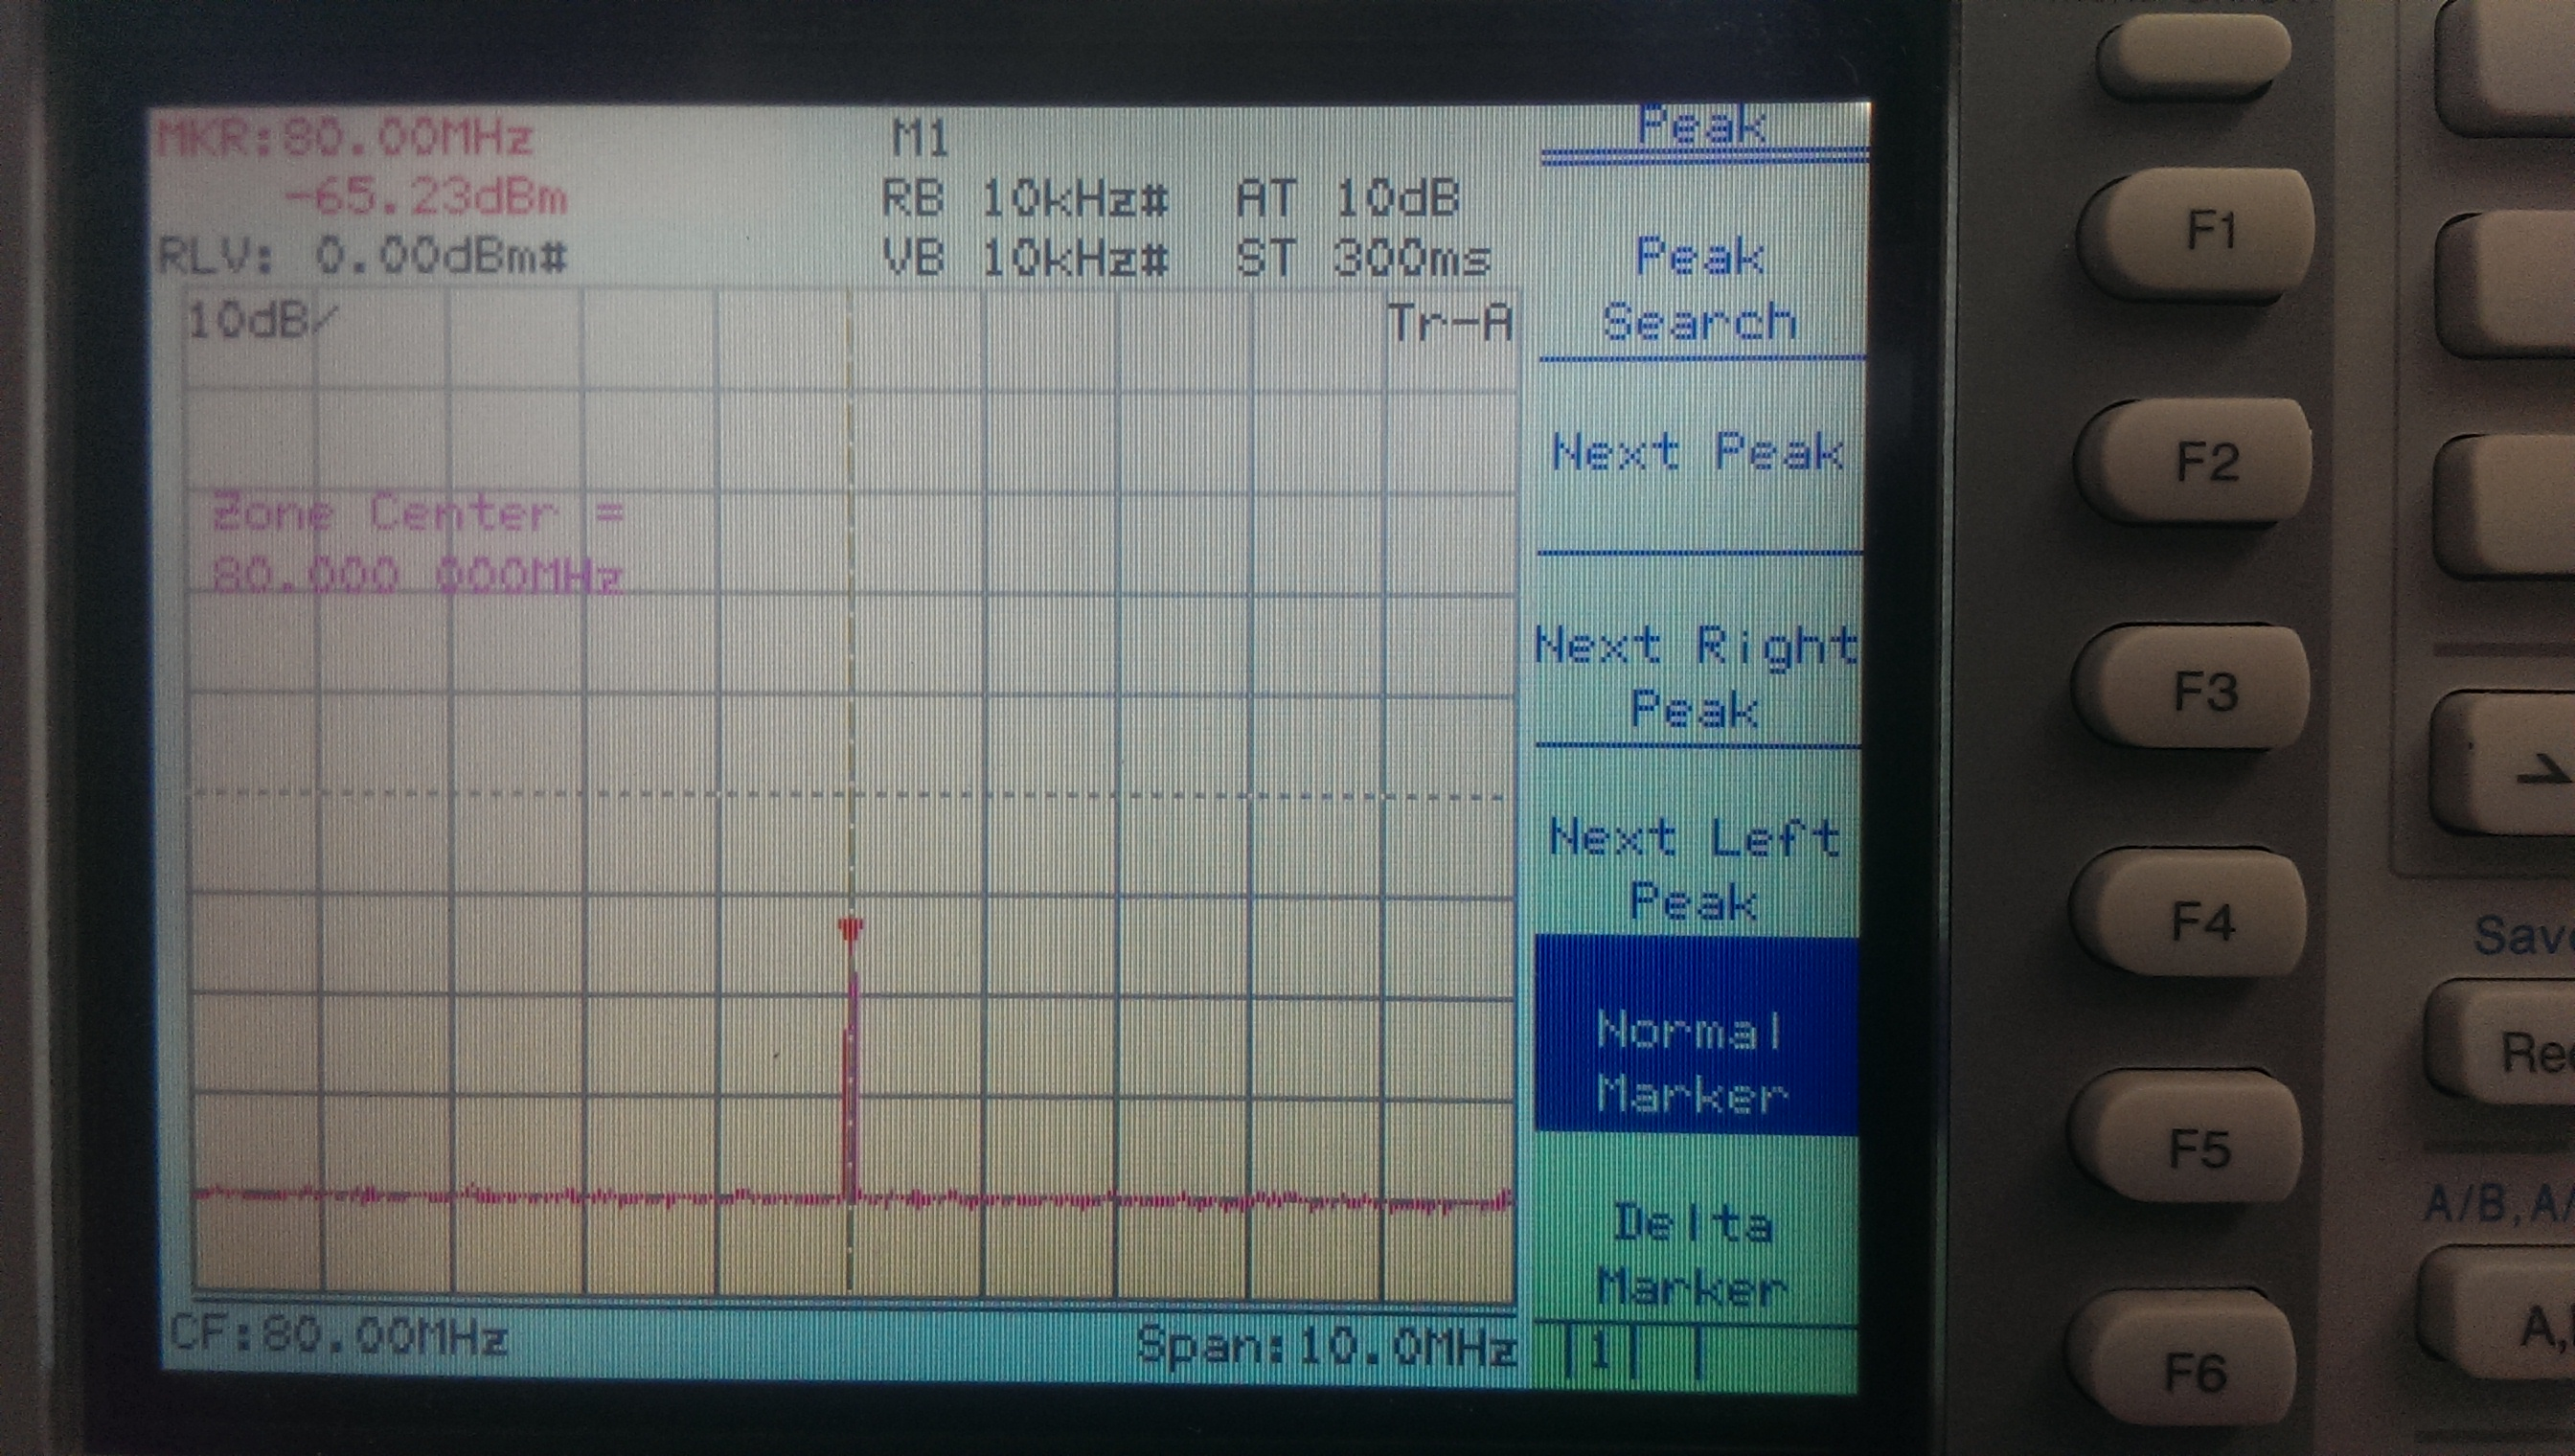
\includegraphics[width=4in]{./images/Figure10.jpg}
		\caption{H-orientation}
		\label{fig:hfield_fig11}
	\end{center}
\end{figure}

